\begin{figure}

\begin{subfigure}{\linewidth}
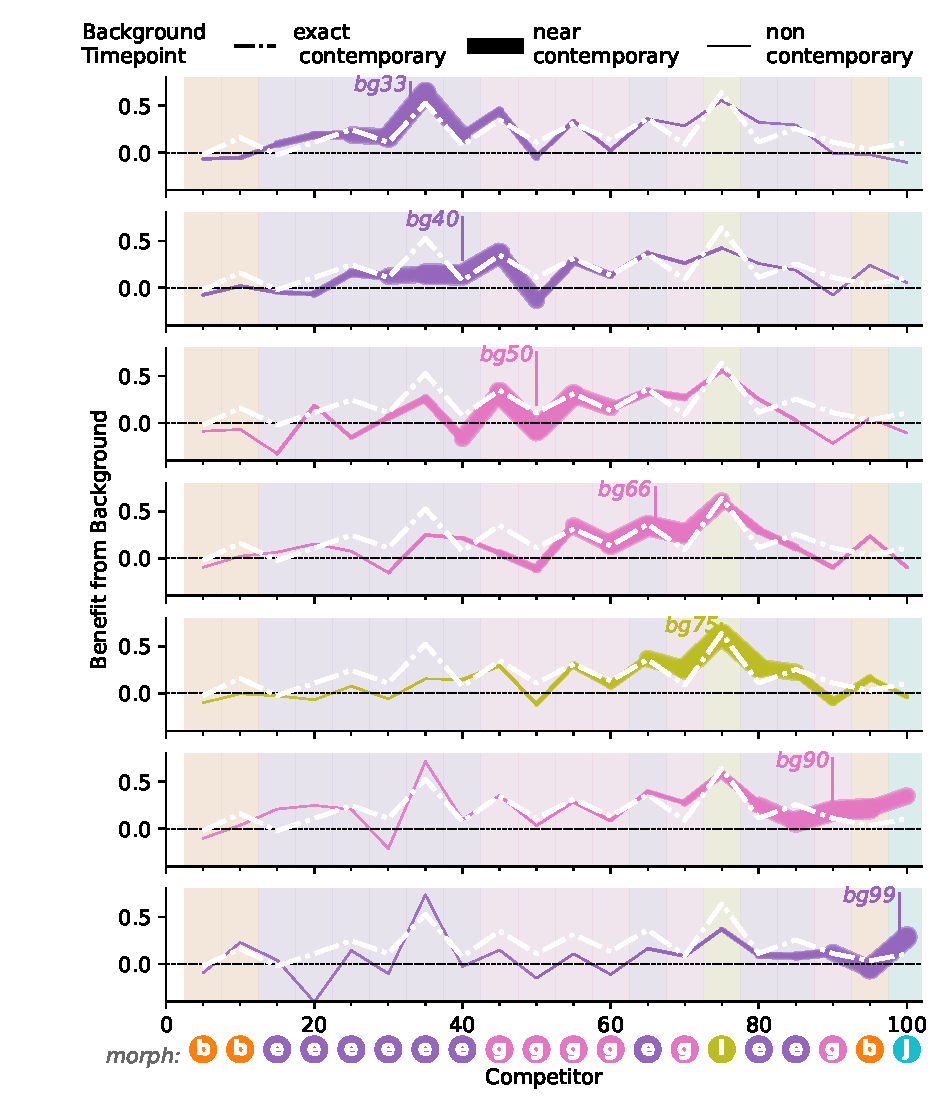
\includegraphics[width=\linewidth]{binder-2025-11-25-external-selfbb-timeshift.ipynb/binder/teeplots/2025-11-25-external-timeshift/viz=subplots+ext=.pdf}

\vspace{-1ex}
\caption{self-context fitness effect of fixed-timepoint backgrounds}
\label{fig:timeshift-full:lineplot}
\end{subfigure}

\begin{subfigure}{\linewidth}

\includegraphics[width=\linewidth]{binder-2025-11-25-external-selfbb-timeshift.ipynb/binder/teeplots/2025-11-25-external-timeshift/hue=isexact+orient=h+viz=swarmplot+x=focal-prevalence+y=isexact+ext=.pdf%
}

\vspace{-1ex}
\caption{timeshift influence on self-context fitness effect}
\label{fig:timeshift-full:swarmplot}
\end{subfigure}

\caption{%
\textbf{Timeshift analysis of self-context fitness effect in case study strain.}
\footnotesize
To assess the evolutionary stability of self-context fitness benefits observed in the case study strain (Figure \ref{fig:fitness-background}), additional fitness assays were conducted with focal strain population samples drawn from stints 33, 40, 50, 66, 75, 90, and 99 as background context (panel \ref{fig:timeshift-full:lineplot}).
Fitness is measured as mean end-state prevalence outcome across ``tournament'' of specimen competition trials between case study strain and focal strain from other independent evolutionary replicates.
Competition is initialized 25/25 between compared strains, with remaining half initialized as a population sample from the case study strain itself (Figure \ref{fig:fit:bbg}).
Color coding indicates morph category of assayed competitor (background fill) and self-context background (line).
Line thickness denotes proximity to self-context background timepoint.
Dashed white overlay shows fitness effect of exact-contemporary self-context background.
Compared against time-shifted effects, exact-contemporary background contexts produced greater fitness benefit (Mann-Whitney $U$ test, panel \ref{fig:timeshift-full:swarmplot}).
}
\label{fig:timeshift-full}

\end{figure}
